\noindent
\section*{Problem 1}

\noindent
\textbf{Manipulation}

In the multiple linear regression, the dependent variable is P/B ratio, the two independent variables are ROE (return on equity) and stock volatility respectively. $i$ represents obserations, i.e. different companies. The time range is 2010Q4. 

The regression result is: : $$P/B_i = 0.1406 + 1.7876 \times ROE_i + 8.6811 \times volatility_i + \epsilon_i$$


\noindent
\textit{Graph.} As shown below, on 2010Q4.
\vspace{5cm}

\begin{figure}[t]
\centering
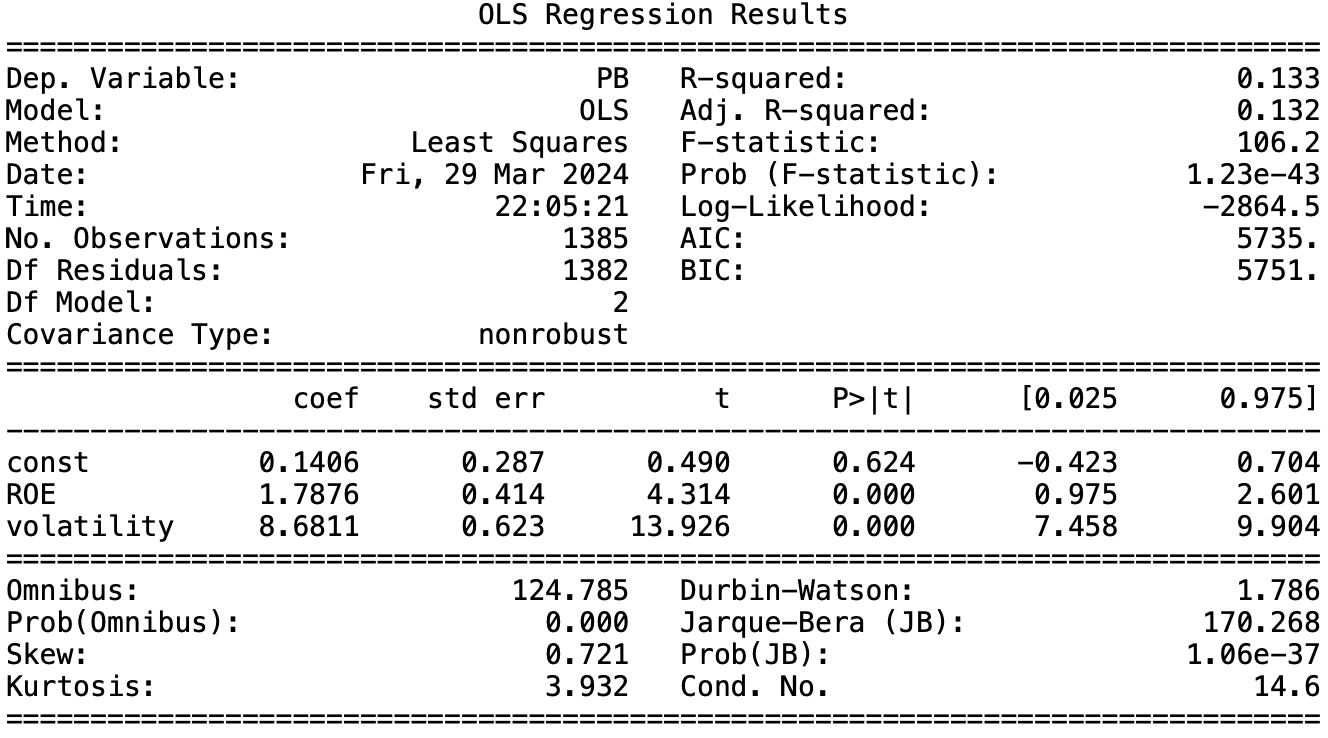
\includegraphics[width=0.85\textwidth]{data/q1_result.png}
\caption{Multiple Linear Regression Results}
\label{fig:example}
\end{figure}


\noindent
\textbf{Regression Results}

Intercept Coefficient (\( \beta_0 \)): The intercept is 0.1406, but it is not statistically significant (p > 0.05), suggesting that when ROE and stock volatility are zero, the P/B ratio is not significantly different from zero.

ROE Coefficient (\( \beta_1 \)): The coefficient for ROE is 1.7876, and it is highly statistically significant $(p < 0.001)$. This means that for each unit increase in ROE, the P/B ratio is expected to increase by approximately 1.7876, holding stock volatility constant.

Volatility Coefficient (\( \beta_2 \)): The coefficient for stock volatility is 8.8611, which is also highly statistically significant $(p < 0.001)$. This suggests that for each unit increase in stock volatility, the P/B ratio is expected to increase by approximately 8.8611, holding ROE constant.

R-squared: The R-squared value is 0.133, which means that approximately 13.3\% of the variation in the P/B ratio is explained by the model. This is a relatively low value, indicating that ROE and volatility cannot explain a large portion of the variability in the P/B ratio.


\noindent
\textbf{Discussion of Findings}

The significant positive relationship between ROE and the P/B ratio suggests that more profitable companies (higher ROE) tend to have a higher P/B ratio.

The significant positive relationship between stock volatility and the P/B ratio suggests that companies with higher stock price volatility are associated with higher P/B ratios. This could be considered to realted to risk premium.

The model's low R-squared value suggests that there are many other factors not included in the model that may also be important in explaining the P/B ratio.

The non-normal distribution of the residuals could be a concern and may indicate that the model's predictions are quite biased or inefficient, so there's still much to improve. But after all, while the model has found statistically significant relationships, we can conclude that P/B ratio is positively related and probably influenced by ROE and stock volatility.


\noindent
\textbf{Possible Reasons}

The P/B ratio can go up when a company's Return on Equity (ROE) increases because a high ROE suggests the company is using its assets efficiently to generate profits. This makes the company more attractive to investors, pushing up its stock price relative to its book value. 

As for volatility, if investors expect higher returns for taking on more risk, a volatile stock with the potential for high returns could see its price increase as investors are willing to pay more, again boosting the P/B ratio. So, in a nutshell, good ROE makes the company look like a money-making champ to investors, and some investors dig the thrill of a roller-coaster stock, willing to bet more money on it, both of which can pump the P/B ratio up.
